\subsection{Listener-System}

\subsubsection{Aufgaben}
Da mit den, von uns unterstützten, Steuerungen nur über das Netzwerk kommuniziert werden kann und sowohl der  \textit{Edubot}- als auch der  \textit{KebaAdapter} laufend Statusupdates von diesen Steuerungen empfangen sollen, muss dieser Datenverkehr parallel zur Ausführung von Befehlen möglich sein.

\subsubsection{Aufbau}
Um diese Aufgabe zu erfüllen werden sogenannter Listener (von “to listen”, horchen) verwendet, welche in einem eigenen Thread auf eingehenden Datenverkehr warten. Da die Art der Vearbeitung dieser Daten von Adapter zu Adapter unterschiedlich sein kann, wurde als Basis der sogenannte INetworkListener implementiert. Dieser kümmert sich um das Empfangen von Daten und gibt die empfangenen Bytes an eine abstrakte Methode weiter, in welcher die Informationen adapterspezifisch verarbeitet werden. Somit muss sich eine, vom  \textit{INetworkListener} abgeleitete, Klasse lediglich auf das Verarbeiten der empfangenen Daten spezialisieren, ohne sich um die Netzwerkkommunikation selbst kümmern zu müssen.

\begin{figure}[H]
  \centering
  \begin{minipage}[t]{12 cm}
  	\centering
  	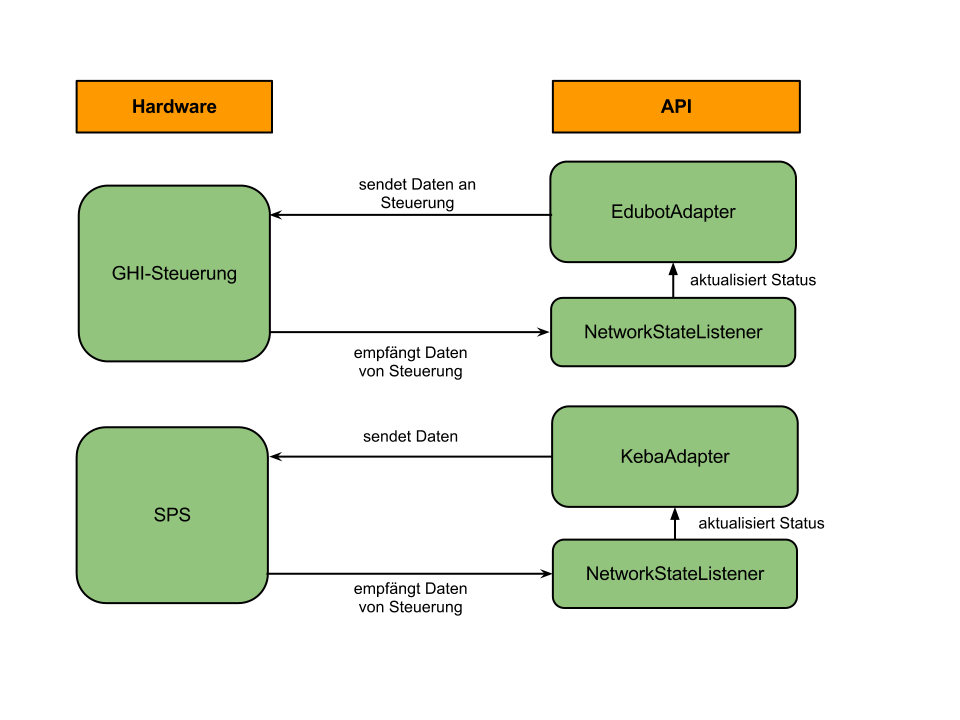
\includegraphics[width=12cm]{images/ListenerSystem} 
    \caption{Listener Konzept}
  \end{minipage}
\end{figure}

\subsubsection{Umsetzung}
\textbf{INetworkStateListener}\\
Die abstrakte Klasse \textit{INetworkStateListener} kümmert sich, wie im Aufbau bereits erwähnt, um das Empfangen von Daten von einer beliebigen Netzwerkschnittstelle. Dazu wird der Klasse im Konstruktor ein, bereits verbundener, Socket mitgegebenen über den Informationen empfangen werden sollen. Weiters ist ein globales Thread-Objekt \textit{listener} definiert welches die \textit{ListenOnState}-Methode im Hintergrund ausführt, wodurch die Netzwerkkommunikation parallel zur restlichen Programmausführung stattfindet.\\
In der \textit{INetworkStateListener}-Klasse sind folgende Methoden implementiert:
\begin{itemize}
\item \textbf{Start}\\
Bei Aufruf der \textit{Start}-Methode wird der Listener-Thread neu instanziert und gestartet. Der  \textit{INetworkStateListener} beginnt ab diesem Zeitpunkt mit dem Empfangen und Weiterleiten von Daten. 
\item \textbf{Stop}\\
Bei Aufruf der \textit{Stop}-Methode wird der aktuell laufende Thread mit Hilfe der  \textit{Abort}-Methode gestoppt und das zugehörige Thread-Objekt auf null gesetzt. Von der Gegenseite gesendete Nachrichten werden nun nicht mehr verarbeitet.
\item \textbf{ListenOnState}\\
Die \textit{ListenOnState}-Methode kümmert sich um das Empfangen und Analysieren von Nachrichten, sowie um das Durchführen der daraus folgenden Status-Updates. 
Die Methode läuft, solange das \textit{IsConnected}-Property der Socket-Klasse true zurückgibt, da dies eine bestehende Verbindung indiziert. Ist der Socket verbunden so wird im nächsten Schritt mit dem \textit{Available}-Property geprüft ob Daten empfangen wurden. Falls auch dieses Property auf \textit{true} gesetzt ist, so werden die bisher empfangenen Bytes mit Hilfe der \textit{Receive}-Methode des Socket gelesen und an einen dynamische Liste angehängt. 
Dieser Vorgang wird solange durchgeführt bis das \textit{Available}-Property \textit{false} zurückliefert, da zu diesem Zeitpunkt die gesamte Nachricht empfangen wurde. Der Inhalt der Liste wird nun durch Aufruf der  \textit{ToArray}-Methode in ein byte[] konvertiert und der \textit{ProcessData}-Methode übergeben. Nachdem diese ausgeführt wurde, wird die Liste geleert und die empfangenen Daten damit verworfen.
\end{itemize}
Die einzige abstrakte Methode des  \textit{INetworkListeners} ist die \textit{ProcessData}-Methode, mit der die Daten individuell verarbeitet werden können.
\begin{itemize}
\item \textbf{ProcessData}\\
Diese Methode wird nachdem vollständigen Empfangen eines Datenblocks durch den Listener-Thread aufgerufen. Die empfangenen Daten werden ihr dabei als Byte-Array übergeben.
\end{itemize}
\\[0.5em]
\textbf{EdubotStateListener}\\
Wie der Name vielleicht vermuten lässt, kümmert sich diese Klasse um die Vearbeitung der, von der GHI-Steuerung empfangenen, Daten. Um Zustandsveränderungen an den entsprechenden \textit{EdubotAdapter} weitergeben zu können, wird dieser im Konstruktor der \textit{EdubotStateListener}-Klasse übergeben.
\begin{itemize}
\item \textbf{ProcessData}\\
Bei Aufruf dieser Methode wird das übergebene Byte-Array mit Hilfe der \textit{Encoding.UTF8.Decode}-Methode in einen String konvertiert und in der Variable \textit{message} gespeichert. Diese wird in einer  \textit{switch}-Kontrollstruktur entsprechend verarbeitet.\\
Handelt es sich bei der empfangenen Nachricht um den String "'ready"' so wird der State des Adapters auf \textit{READY} gesetzt und damit der nächste Befehle aus der Warteschlange, falls einer vorhanden ist, ausgeführt.
Wird der String "'shutdown"' empfangen, indiziert dies das erfolgreiche Herunterfahren des Roboters und der \textit{State} des Adapters wird auf \textit{SHUTDOWN} gesetzt. Sollte die empfangene Nachricht mit "'err:"' beginnen, so bedeutet dies das ein Fehler auf der Steuerung aufgetreten ist und das \textit{OnFailure}-Event des entsprechenden Adapters wird ausgelöst. Dabei wird die empfangene Nachricht als Event-Argument mitgegeben, da sie detailliertere Informationen zum aufgetretenen Fehler enthält.
\end{itemize}
\\[0.5em]
\textbf{KebaStateListener}\\
Um in Bezug auf zukünftige Erweiterungen der Funktionen des KebaAdapters flexibel zu bleiben, wurde auch für diesen eine eigene, vom  \textit{INetworkStateListener} abgeleitete, Klasse entwickelt. Derzeit ist der einzige Unterschied zum  \textit{EdubotStateListener} der übergebene Adaptertyp, da es sich hierbei logischerweise um ein  \textit{KebaAdapter}-Objekt handelt.
\begin{itemize}
\item \textbf{ProcessData}\\
Bei Aufruf dieser Methode wird das übergebene Byte-Array mit Hilfe der \textit{Encoding.UTF8.Decode}-Methode in einen String konvertiert und in der Variable \textit{message} gespeichert. Diese wird in einer  \textit{switch}-Kontrollstruktur entsprechend verarbeitet.\\
Handelt es sich bei der empfangenen Nachricht um den String "'ready"' so wird der State des Adapters auf \textit{READY} gesetzt und damit der nächste Befehle aus der Warteschlange, falls einer vorhanden ist, ausgeführt.
Wird der String "'shutdown"' empfangen, indiziert dies das erfolgreiche Herunterfahren des Roboters und der \textit{State} des Adapters wird auf \textit{SHUTDOWN} gesetzt. Sollte die empfangene Nachricht mit "'err:"' beginnen, so bedeutet dies das ein Fehler auf der Steuerung aufgetreten ist und das \textit{OnFailure}-Event des entsprechenden Adapters wird ausgelöst. Dabei wird die empfangene Nachricht als Event-Argument mitgegeben, da sie detailliertere Informationen zum aufgetretenen Fehler enthält.
\end{itemize}